\section{Motivation}
\label{s:motivation}

% - characteristics of concurrency bugs
% - challenges / design requirements
% - limitations of existing approaches

This work is motivated by an observation that none of previous works
properly addresses characteristics of \textit{offending thread
  interleaving} (\ie, one that causes a concurrency bug).
%
As a consequence, previous works either \textbf{1)} suffer from
identifying whether interesting thread interleavings remain
untested~\cite{krace, conzzer, muzz}, or \textbf{2)} waste the
computing power by ineffectively exploring the search space of thread
interleaving~\cite{snowboard, razzer}.



In this section, we first comprehend why concurrency bugs manifest
depending on thread interleaving through a real-world concurrency bug
example.
%
We then define design goals for effectively discovering concurrency
bugs in the kernel, and summarize why existing approaches fall short
in satisfying the design goals.


\PP{Manifestation of concurrency bugs}
%
\begin{figure}[t]
  \centering
  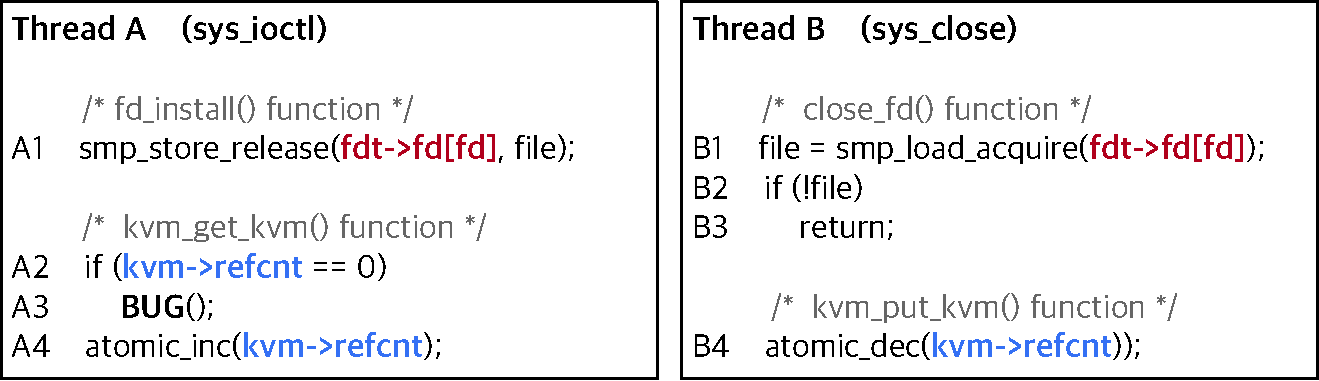
\includegraphics[width=0.9\linewidth]{fig/cve-2017-10661.pdf}
  \caption{Simplified code snippet of CVE-2017-17712. If \texttt{B1}
    is executed between \texttt{A2} and \texttt{A4}, concurrenct
    accesses on \texttt{inet->hdrincl} leads to uninitialized stack
    pointer usage on \texttt{rfv}, and an attacker may gain root
    privileges through a dedicated attack
    technique~\cite{stackspray}.\yj{I do not know how attacker can
      gain a root privilege}}
  \label{fig:cve-2017-17712}
\end{figure}
%
In \autoref{fig:cve-2017-17712}, an uninitialized access bug, which
may allow attackers to gain root privileges, may manifest when two
system calls are executed concurrently: \texttt{sendmsg()} to send a
message through an ipv4 socket, and \texttt{setsockopt()} to modify an
option of the ipv4 socket.
%
Assuming \texttt{inet->hdrincl} is initially \texttt{1}, the
concurrency bug manifests depending on the execution order of three
memory accesses, \texttt{A2} and \texttt{A4} in thread~A, and
\texttt{B1} in thread~B.
%
During sending a message through the ipv4 socket, thread~A reads a
value of \texttt{inet->hdrincl} twice at \texttt{A2} and \texttt{A4}.
%
However, since these two read operations are not atomically executed,
thread~B may intervene in the middle of these two read operations.
%
In that case, if \texttt{B1} is executed between \texttt{A2} and
\texttt{A4}, thread~A reads different values of \texttt{inet->hdrincl}
at \texttt{A2} and \texttt{A4}, and dereference \texttt{rfv} without
initializing it.


\PP{Observation 1: Combined interleaving orders}
%
This example demonstrates that a concurrency bug is \textit{a combined
  result of a few interleaving orders}, where each interleaving order
denotes the execution order between an instruction pair that access
the same memory object.
%
In the example of \autoref{fig:cve-2017-17712}, two interleaving orders
are required to cause the uninitialized access bug.
%
First, \texttt{A2} should be executed before \texttt{B1} (\ie,
$\texttt{A2} \Rightarrow \texttt{B1}$\footnote{In this paper,
  $\texttt{X} \Rightarrow \texttt{Y}$ denotes that \texttt{X} is
  executed before \texttt{Y}}) to make thread~A not initialize
\texttt{rfv}.
%
Second, \texttt{B1} should be executed before \texttt{A4} (\ie,
$\texttt{B1} \Rightarrow \texttt{A4}$) to make thread~A dereference
uninitialized \texttt{rfv}.
%
Therefore, thread interleavings that satisfy a combination of two
interleaving orders (\ie,
$\texttt{A2} \Rightarrow \texttt{B1} \Rightarrow \texttt{A4})$ cause
the uninitialized access bug, while all other thread interleavings do
not.


\PP{Design goal 1: Combinatorial interleaving coverage}
%
As shown in the above observation, a concurrency bug is not caused by
just a single interleaving order (\eg,
$\texttt{A2} \Rightarrow \texttt{B1}$), but by a combination of
interleaving orders (\eg,
$\texttt{A2} \Rightarrow \texttt{B1} \Rightarrow \texttt{A4}$).
%
As a consequence, tracking individual interleaving orders is not
enough as an interleaving coverage metric.

\begin{figure}[t]
  \centering
  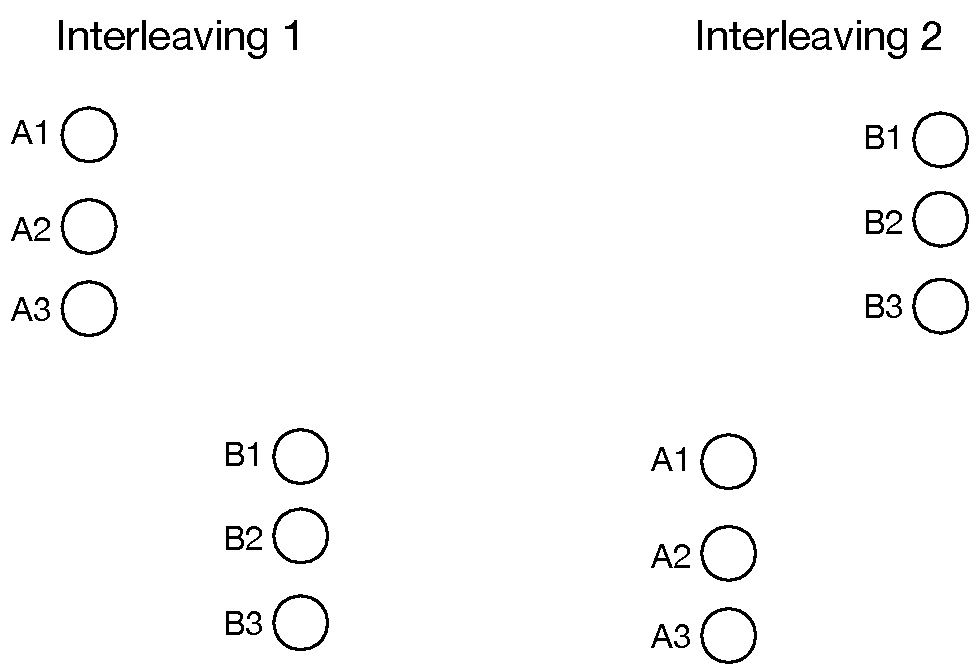
\includegraphics[width=0.95\linewidth]{fig/alias-coverage.pdf}
  \caption{Two thread interleavings between thread~A and thread~B
    described in \autoref{fig:cve-2017-17712}. The uninitialized
    access bug does not manifest in both interleavings.}
  \label{fig:alias-coverage}
\end{figure}
%
\autoref{fig:alias-coverage} shows what happens if an interleaving
coverage metric tracks individual interleaving orders.
%
In the two interleavings described in this figure, we can observe all
four individual interleaving orders regarding \texttt{inet->hdrincl}
(\ie, $\texttt{A2} \Rightarrow \texttt{B1}$ and
$\texttt{A4} \Rightarrow \texttt{B1}$ in Interleaving~\#1,
$\texttt{B1} \Rightarrow \texttt{A2}$, and
$\texttt{B1} \Rightarrow \texttt{A4}$ in Interleaving~\#2), while the
uninitialized access bug does not manifest in both thread
interleavings.
%
Therefore, if an interleaving coverage metric tracks individual
interleaving orders, the coverage metric can be saturated even though
a concurrency bug still resides in a multi-thread input, and a fuzzer
may miss a concurrency bug.
%
To avoid this pitfall, an interleaving coverage metric should be
designed while considering a combination of interleaving orders.




% In the example of \autoref{fig:cve-2017-17712}, \textbf{R1} states
% that if the two system calls (\ie, \texttt{sendmsg()} and
% \texttt{setsockopt()}) no longer give new interleaving coverage with
% respect to a given interleaving coverage metric (\ie, interleaving
% coverage is saturated), a fuzzer will de-prioritize the two system
% calls to explore thread interleavings of another multi-thread input.
% %
% Therefore, in order not to miss the uninitialized access bug, an
% interleving coverage metric should be able to capture whether

% $(\texttt{A2} \Rightarrow \texttt{B1}) \wedge (\texttt{B1} \Rightarrow
% \texttt{A4})$ is tested or not.
% %
% Otherwise, a fuzzer cannot decide if two more system calls need to be executed.
% Therefore, the uninitialized access bug may be missed 


\PP{Observation 2: Feedback from previous executions}
%
Interestingly, a previous execution that did not cause the
uninitialized access bug provides a feedback as to which thread
interleavings should be further explored.
%
To demonstrate this, let us assume we execute the two system calls
\textit{sequentially} such that the execution of thread~A is followed
by the execution of thread~B.
%
Even though the sequential execution does not cause the uninitialized
access bug, we can observe that three instructions, \texttt{A2},
\texttt{A4}, and \texttt{B1} are executed in the order of
$\texttt{A2} \Rightarrow \texttt{A4} \Rightarrow \texttt{B1}$.
%
Unsuprisingly, we can easily imagine an interleaving of these three
instructions by flipping the execution order of \texttt{A4} and
\texttt{B1} (\ie,
$\texttt{A2} \Rightarrow \texttt{B1} \Rightarrow \texttt{A4}$).
%
And this imaginary interleaving is what exactly we are looking for; it
is the condition that causes the uninitialized access bug, and if we
execute the imaginary interleaving, we can discover the uninitialized
access bug.



\PP{Design goal 2: History-directed thread scheduling control}
%
Based on the observation 2, we elicit a design goal of a thread
scheduling control mechanism.
%
Particulary, a thread scheduling control mechanism should leverage a
history of previous executions to efficiently determine what to search
in future executions.

Since thread interleaving is inherently non-deterministic, blindly
repeating the execution of two system calls in
\autoref{fig:cve-2017-17712} will likely waste the computing power
without making a progress of the thread interleaving exploration.





%
% \textbf{R2} describes that if this combined interleaving orders has
% not been tested, a fuzzer needs to schedule instructions to quickly
% cover the combined interleaving orders instead of exploring the entire
% search space of thread interleaving randomly.


\subsection{Limitation of prior approaches}
\label{ss:existingapproaches}

\yj{Revise hint: Flow-OK, Clarification of text-Need work}
\begin{table}[t]
  \centering
  \resizebox{\linewidth}{!}{
  \begin{tabular}{l l l}
    \toprule
    & \thead{\textbf{Interleaving} \\ \textbf{coverage metric}} & \thead{\textbf{Interleaving} \\ \textbf{search strategy}} \\
    \midrule
    \textbf{Razzer~\cite{razzer}} & -- & Coverage-oblivious \\
    \textbf{Krace~\cite{krace}} & Alias coverage & Coverage-oblivious \\
    % & (single instruction pair) & \\
    \textbf{Conzzer~\cite{conzzer}} & Concurrent call pair & Coverage-based (limited) \\
    % & (single function pair) & (limited)\\
    \textbf{Snowboard~\cite{snowboard}} & -- & Coverage-oblivious \\
    \bottomrule
  \end{tabular}
}

%%% Local Variables:
%%% mode: latex
%%% TeX-master: "../p"
%%% End:

  \caption{Recent fuzzing works to discover concurrency bugs in the
    kernel, and their interleaving coverage metrics (\textbf{R1}) and
    thread scheduling control mechanisms (\textbf{R2}). ``--''
    indicates that a fuzzer does not adopt a concurrency coverage
    metric.}
  \label{table:motivation}
\end{table}

As shown in \autoref{table:motivation}, prior concurrency fuzzing
approaches adopt different interleaving coverage metrics and thread
scheduling control mechanisms.
%
Even though prior approaches achieve their own successes, we find that
their interleaving coverage metrics and thread scheduling control
mechanisms do not satisfy \textbf{Design goal 1} and \textbf{2}.


\PP{Insufficient coverage metric}
%
%
We find that none of existing interleaving coverage metrics consider
a combination of interleaving orders.
%
Therefore, they are not sufficient to determine whether interesting
(\ie, offending) thread interleaving remains untested. Thus, they do
not satisfy \textbf{R1}.


In particular,


after KRace~\cite{krace} first emphasizes the necessity
of a coverage metric in the concurrency dimension, different
concurrency coverage metrics are proposed such as \textit{alias
  coverage}~\cite{krace}, \textit{concurrent call
  pair}~\cite{conzzer}, and \textit{\dr{TODO: MUZZ
    coverage}}~\cite{muzz}.
%
\yj{This paragraph must be easy enough for reader to intuitively understand, but hard to digest discussions}
However, they are not applicable to track behavioral changes\yj{what does it mean?} according
to a combination of interleaving orders, mainly because they either
track only a \textit{single} interleaving order~\cite{krace, muzz} or
\textit{coarse-grained information} such as a pair of two
concurrently-executed functions~\cite{conzzer}.
\yj{I do not understand why tracking a single int. order and coarse-grain information are not able to track behavioral changes}

Taking the example of KRace's alias coverage,
\autoref{fig:alias-coverage} describes two thread interleavings that
saturate alias coverage found between two system calls in
\autoref{fig:cve-2017-17712}.
%
In these example interleaving scenarios, the uninitialized access does
not manifest even after alias coverage is saturated, and a fuzzer may
decide to stop searching for new thread interleavings in the two
system calls.
%
While we do not enumerate all proposed interleaving coverage metrics
here, we find that they all share the same limitation.


\PP{Ineffective scheduling mechanism}
%
Stemming from insufficient coverage metrics, proposed scheduling
mechanisms are also ineffective in satisfying \textbf{R2}.
%
As described in \autoref{s:background}, proposed scheduling mechanisms
are largely categorized into two: a randomized scheduler and a
hint-directed scheduler.

\dr{revisit after evaluation. not ready to write this part:}
%
Randomized schedulers~\cite{krace, pctalgorithm, muzz, ski} pay little
attention on collected interleaving coverage when scheduling
instructions, and rely on the randomness in diversifying thread
interleaving.
%
Therefore, they are inherently limited in satisfying a specific
condition of thread interleaving (\eg,
$(\texttt{A2} \Rightarrow \texttt{B1}) \wedge (\texttt{B1} \Rightarrow
\texttt{A4})$ in \autoref{fig:cve-2017-17712}).
%
This limitation is even more pronounced by a recent study,
ExpRace~\cite{exprace}, stating that many concurrency
bugs~\cite{cve20196974, cve20191999, cve201911486} manifest only if
thread interleaving satisfies an extreme condition that randomized
scheduler hardly satisfy.
%
Unfortunately, ExpRace demonstrates that this kind of concurrency bugs
are equally threatening the security of the kernel.


Whereas, state-of-the-art approaches adopting a hint-directed
scheduler, Razzer~\cite{razzer} and Snowboard~\cite{snowboard}, are
not capable of diversifying thread interleaving across iterations.
%
Since they do not adopt interleaving coverage, they are not able to
determine which thread interleaving requires further
testing. Therefore, they vary thread interleaving a small degree
across fuzzing iterations, and require a long time to trigger
concurrency bugs.
%
According to our evaluation~\autoref{s:eval}, ...


% In the perspective of fuzzing, a coverage metric is a paramount gear
% to determine whether a given input is worthy of further mutation.
% %
% If a coverage metric does not represent whether an input has a
% potential to trigger a race condition, a fuzzer may ignore inputs in
% which there are unexplored interleavings, or waste the computing power
% to valueless inputs.
% %
% In this regard, our primary question is whether existing coverage
% metrics in the concurrency dimension are suitable to apprehend
% interleavings potentially causing a race condition, for example,
% $(\texttt{A1} \Rightarrow \texttt{B1}) \wedge (\texttt{B4} \Rightarrow
% \texttt{A2})$ in \autoref{fig:cve-2017-17712}.



% Unfortunately, we observe that none of existing approaches incorporate
% a proper coverage metric for race conditions.
% %
% A few of existing approaches~\cite{snowboard, razzer} do not adopt a
% coverage in the concurrency dimension at all. Therefore, they do not
% make a decision as to whether a given input is worth further testing.
% %
% Other approaches~\cite{krace, muzz} adopt coverage metrics that are
% not suitable for race conditions as they do not consider a combined
% result of multiple pairs of conflicting accesses. As a consequence,
% race conditions may not be exposed even after the coverages are
% saturated.
% %
% % Consequently, existing approaches have difficulty in distinguishing a
% % given input has a potential to cause an interesting behavior, \ie,
% % a race condition.



% \yj{This is the key paragraph to point out the limitation of previous approaches, but very vague. Make specific claims of why Kraces' alias coverage is insufficient by giving an example.}
% %
% In order to show why comprehending multiple pairs of conflicting
% accesses is important, let us suppose we have three inputs that
% consists of two concurrent syscalls as described in
% \autoref{fig:alias-coverage}.
% %
% For all inputs, thread~A executes a \texttt{mmap()} syscall to map the
% binder driver to a user address space while thread~B handles different
% ioctl requests such that \texttt{ioctl(FREE_BUFFER)},
% \texttt{ioctl(REPLY)}, and \texttt{ioctl(TRANSACTION)} for
% \texttt{Input 1}, \texttt{Input 2}, and \texttt{Input 3} respectively.
% %
% It is worth noting that in \texttt{Input 1} and \texttt{Input 2},
% there is only one pair of conflicting accesses; in \texttt{Input 1},
% the two threads conflict on \texttt{alloc->vma}, and in \texttt{Input
%   2}, the two threads conflict on \texttt{alloc->mm}.



% \begin{figure}[t]
%   \centering
%   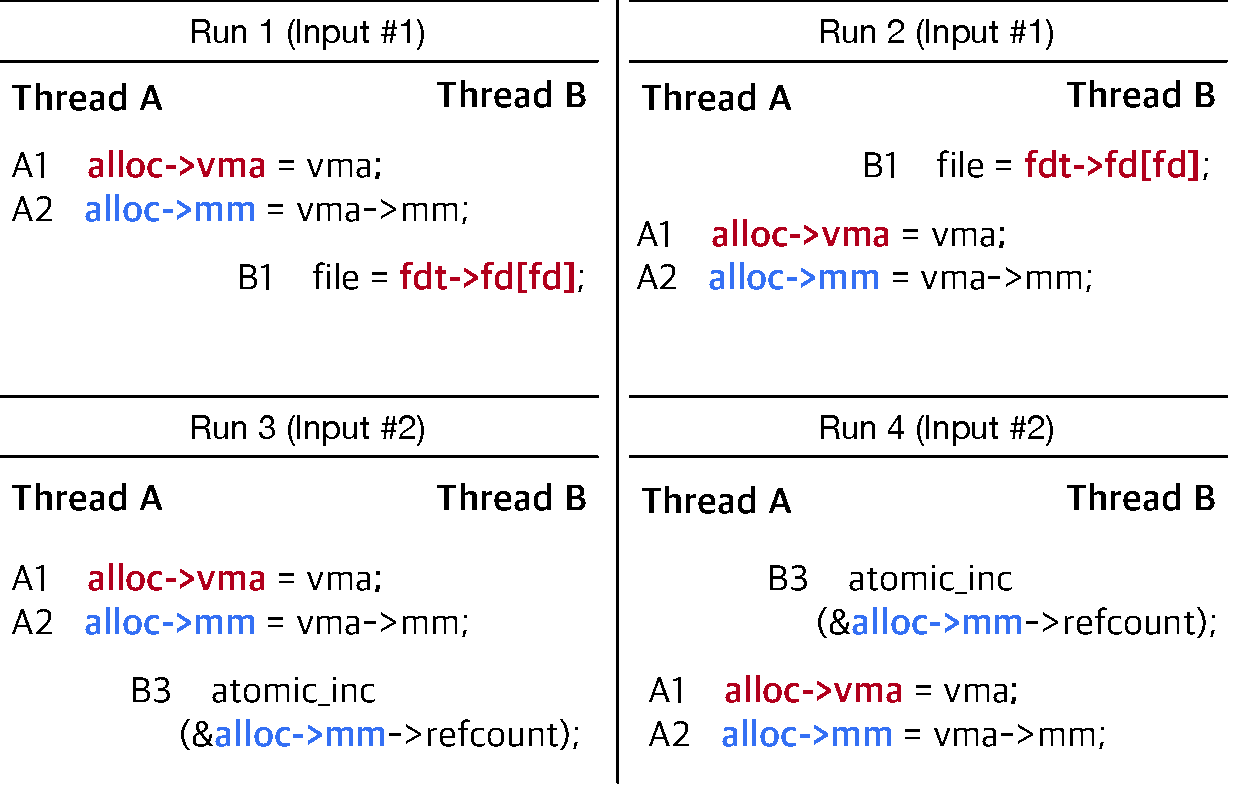
\includegraphics[width=0.9\linewidth]{fig/alias-coverage-interleaving.pdf}
%   \caption{Four interleavings of \texttt{Input 1} and \texttt{Input 2}
%     in \autoref{fig:alias-coverage}. After executing these four
%     interleavings, all possible execution orders of a single
%     conflicting accesses are exhibited.\dr{Run 1 -> Interleaving 1?}}
%   \label{fig:alias-coverage-interleaving}
% \end{figure}

% In this example, if we adopt a coverage metric that focuses on a
% single pair of conflicting accesses (\eg, alias coverage), a fuzzer
% may not recognize that \texttt{Input 3} may exhibit a different
% behavior than \texttt{Input 1} and \texttt{Input 2}~(\ie, a
% NULL-dereference bug).
% %
% \autoref{fig:alias-coverage-interleaving} shows four interleavings
% that exhibits all execution order of a single pair of conflicting
% accesses. If a fuzzer executes \texttt{Input 1} with interleavings in
% \texttt{Run 1} and \texttt{Run 2}, a fuzzer observes execution orders
% such as $\texttt{A1} \Rightarrow \texttt{B1}$ (in \texttt{Run 1}) and
% $\texttt{B1} \Rightarrow \texttt{A1}$ (in \texttt{Run 2}).
% %
% Similary, if a fuzzer executes \texttt{Input 2} with interleavings in
% \texttt{Run 3} and \texttt{Run 4}, it observes execution orders of
% $\texttt{A2} \Rightarrow \texttt{B4}$ (in \texttt{Run 3}) and
% $\texttt{B4} \Rightarrow \texttt{A2}$ (in \texttt{Run 4}).
% %
% After executing these four interleavings, \texttt{Input 3} does not
% reveal a new execution order of a single conflicting
% accesses. Therfore, as a Krace state, a fuzzer may de-prioritize
% \texttt{Input 3}, and the race condition may not be found.

% In summary, in order to determine whether an input shows interesting
% behaviors or not, a fuzzer needs to comprehend \textit{a combined
%   result of multiple pairs of conflicting accesses} as it is the
% primary reason of race conditions.



%%% Local Variables:
%%% mode: latex
%%% TeX-master: "p"
%%% End:
